\begin{minipage}{0.75\linewidth}
\begin{figure}[h]
    \centering
    \begin{adjustbox}{max width=1.0\linewidth, keepaspectratio}
        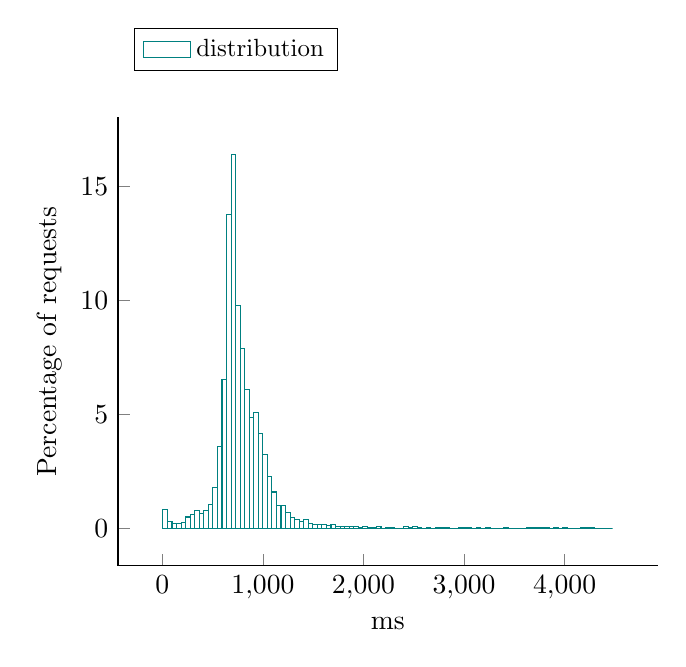
\begin{tikzpicture}
            \begin{axis}[ylabel = Percentage of requests, 
xlabel = ms, 
legend style = {nodes={scale=0.9, transform shape}, at={(0.03,1.2)}, anchor=north west, draw=black, fill=white, align=left, legend columns=3},
area style, mark size = 0pt,
 cycle list name = exotic,
  axis lines* = left]
		\addplot +[ybar interval] coordinates {
			 (5, 0.837729)
			 (50.18, 0.31027)
			 (95.36, 0.206847)
			 (140.54, 0.206847)
			 (185.72, 0.268901)
			 (230.9, 0.496432)
			 (276.08, 0.62054)
			 (321.26, 0.786017)
			 (366.44, 0.641225)
			 (411.62, 0.775675)
			 (456.8, 1.05492)
			 (501.98, 1.79957)
			 (547.16, 3.5681)
			 (592.34, 6.52601)
			 (637.52, 13.7553)
			 (682.7, 16.3823)
			 (727.88, 9.7735)
			 (773.06, 7.8912)
			 (818.24, 6.08129)
			 (863.42, 4.87124)
			 (908.6, 5.08843)
			 (953.78, 4.14727)
			 (998.96, 3.24749)
			 (1044.14, 2.27531)
			 (1089.32, 1.59272)
			 (1134.5, 0.982521)
			 (1179.68, 0.992864)
			 (1224.86, 0.692936)
			 (1270.04, 0.465405)
			 (1315.22, 0.372324)
			 (1360.4, 0.31027)
			 (1405.58, 0.372324)
			 (1450.76, 0.196504)
			 (1495.94, 0.165477)
			 (1541.12, 0.17582)
			 (1586.3, 0.155135)
			 (1631.48, 0.124108)
			 (1676.66, 0.17582)
			 (1721.84, 0.0723963)
			 (1767.02, 0.093081)
			 (1812.2, 0.0827386)
			 (1857.38, 0.0723963)
			 (1902.56, 0.0723963)
			 (1947.74, 0.0206847)
			 (1992.92, 0.062054)
			 (2038.1, 0.0413693)
			 (2083.28, 0.0517117)
			 (2128.46, 0.062054)
			 (2173.64, 0.0103423)
			 (2218.82, 0.031027)
			 (2264, 0.031027)
			 (2309.18, 0.0103423)
			 (2354.36, 0)
			 (2399.54, 0.0723963)
			 (2444.72, 0.0517117)
			 (2489.9, 0.062054)
			 (2535.08, 0.0413693)
			 (2580.26, 0.0103423)
			 (2625.44, 0.0206847)
			 (2670.62, 0.0103423)
			 (2715.8, 0.0413693)
			 (2760.98, 0.0206847)
			 (2806.16, 0.0206847)
			 (2851.34, 0)
			 (2896.52, 0)
			 (2941.7, 0.0413693)
			 (2986.88, 0.031027)
			 (3032.06, 0.031027)
			 (3077.24, 0.0103423)
			 (3122.42, 0.0517117)
			 (3167.6, 0)
			 (3212.78, 0.0206847)
			 (3257.96, 0.0103423)
			 (3303.14, 0.0103423)
			 (3348.32, 0)
			 (3393.5, 0.031027)
			 (3438.68, 0.0103423)
			 (3483.86, 0)
			 (3529.04, 0)
			 (3574.22, 0)
			 (3619.4, 0.031027)
			 (3664.58, 0.0206847)
			 (3709.76, 0.0206847)
			 (3754.94, 0.0206847)
			 (3800.12, 0.0206847)
			 (3845.3, 0.0103423)
			 (3890.48, 0.031027)
			 (3935.66, 0)
			 (3980.84, 0.031027)
			 (4026.02, 0.0103423)
			 (4071.2, 0)
			 (4116.38, 0)
			 (4161.56, 0.0206847)
			 (4206.74, 0.0206847)
			 (4251.92, 0.0206847)
			 (4297.1, 0.0103423)
			 (4342.28, 0.0103423)
			 (4387.46, 0.0103423)
			 (4432.64, 0)
			 (4477.82, 0)
		};
\addlegendentry{distribution};
           \end{axis}
      \end{tikzpicture}
  \end{adjustbox}
  \caption{Response time distribution - req = ReadUser-2}
\end{figure}
\end{minipage}\hfill\begin{minipage}{0.18\linewidth}
\begin{table}[h]
\begin{tabular}{|cc|}
\hline
\textbf{} & \textbf{ms}\\ \hline
 \Xhline{0.005\arrayrulewidth}
min & 5\\
 \Xhline{0.005\arrayrulewidth}
max & 4523\\
 \Xhline{0.005\arrayrulewidth}
mean & 799\\
 \Xhline{0.005\arrayrulewidth}
std & 338\\
\hline
\hline
 \Xhline{0.005\arrayrulewidth}
25th & 663\\
 \Xhline{0.005\arrayrulewidth}
50th & 733\\
 \Xhline{0.005\arrayrulewidth}
75th & 892\\
 \Xhline{0.005\arrayrulewidth}
80th & 937\\
 \Xhline{0.005\arrayrulewidth}
85th & 985\\
 \Xhline{0.005\arrayrulewidth}
90th & 1056\\
 \Xhline{0.005\arrayrulewidth}
95th & 1212\\
 \Xhline{0.005\arrayrulewidth}
99th & 2169\\
\hline
\end{tabular}
\caption{Response time}
\end{table}
\end{minipage}\hfill